\documentclass[12pt]{article}
\usepackage{graphicx}
\usepackage{hyperref}
\usepackage[round]{natbib}
\bibliographystyle{agsm}
\usepackage{geometry}
\geometry{margin=1in}
\title{AI-Based News Summarization: Leveraging Natural Language Processing for Extractive and Abstractive Summaries}
\author{
    Stanley Osei-Wusu\\
    Gisma University of Applied Sciences, Potsdam, Germany\\
    stanley.osei-wusu@gisma-student.com\\GH1021715
}
\date{\today}

\begin{document}

\maketitle
\newpage
\begin{abstract}
In the digital era, there is a growing need for efficient methods to process and consume news. This paper presents an AI-based system designed to automate the summarization of news articles using both extractive and abstractive techniques. The proposed system leverages state-of-the-art transformer models to summarize news content from multiple sources, such as NewsAPI, BBC, CNN, Reuters, and Daily Mail, and publishes the results on a WordPress blog. The system automates the end-to-end workflow, from data fetching and text preprocessing to summarization and publication. The experiment shows that the system is highly effective at summarizing large volumes of news articles, providing concise, accurate, and human-like summaries. Deployment results on real-world platforms have demonstrated the potential of the system in the field of automated news summarization.
\end{abstract}

\section{Introduction}
The massive influx of digital news content poses challenges for individuals and organizations in efficiently consuming information. News summarization addresses this challenge by providing concise summaries that capture the essence of the full article. Traditionally, summarization has been performed manually, but advances in artificial intelligence and natural language processing (NLP) have made it possible to automate this process \citep{manning1999foundations}. This work presents an AI-based system for news summarization that uses extractive and abstractive techniques to generate high-quality summaries from news articles. The system fetches articles from NewsAPI \citep{newsapi} and sources such as BBC, CNN, Reuters, and Daily Mail, processes the text, and generates summaries that are automatically posted on a WordPress blog.

\section{Problem Statement}
\subsection{Business Problem}
The client, a news aggregation platform, aims to provide concise summaries of news articles to improve user engagement and retention. With the overwhelming amount of digital news content, users struggle to keep up with current events. This summarization system will help users save time by providing the most important details in a summarized format.

\subsection{Importance of the Problem}
Providing efficient news summaries is crucial for:
\begin{itemize}
    \item \textbf{User Engagement}: Concise summaries enhance the user experience by allowing users to quickly grasp the key points.
    \item \textbf{Combating Information Overload}: Summarization mitigates the effects of information overload by providing relevant and filtered content.
    \item \textbf{Competitive Advantage}: Offering high-quality summaries can help differentiate the platform from competitors.
\end{itemize}

\subsection{Data Collection}
The system collects data from various sources, including:
\begin{itemize}
    \item \textbf{News APIs}: The NewsAPI is utilized to fetch articles from multiple news sources, including BBC, CNN, Reuters, and Daily Mail \citep{newsapi}.
    \item \textbf{Web Scraping}: Scraping tools are used to extract text from websites that are not directly accessible via APIs.
\end{itemize}

\section{System Design}
\subsection{High-Level Overview}
The system consists of several components that are connected in a pipeline to automate the end-to-end summarization process:
\begin{itemize}
    \item \textbf{Data Collection Module}: Collects articles from multiple sources.
    \item \textbf{Preprocessing Module}: Cleans and tokenizes the text to prepare it for summarization.
    \item \textbf{Summarization Module}: Performs both extractive and abstractive summarization to generate concise summaries \citep{raffel2020exploring}.
    \item \textbf{Evaluation Module}: Evaluates the quality of the summaries using metrics such as ROUGE.
    \item \textbf{Publishing Module}: Automatically posts summaries to a WordPress blog.
\end{itemize}

\subsection{News Summarizer Workflow Diagram}
This diagram illustrates the end-to-end workflow of the application, from fetching news articles to posting on the WordPress blog.

\begin{figure}[htbp]
    \centering
    \includegraphics[width=0.8\textwidth]{Copy of News summarizer workflow chart.png}
    \caption{News Summarizer Application Workflow}
    \label{fig:workflow}
\end{figure}

\newpage
\section{Detailed Design, Implementation, and Analysis}
Each module plays a critical role in the summarization pipeline:

\subsection{Data Collection Module}
This module fetches raw news articles via APIs or web scraping techniques. The data collection module interfaces with NewsAPI to retrieve articles and metadata, such as titles, descriptions, and publication dates \citep{newsapi}.

\subsection{Preprocessing Module}
Text preprocessing is crucial for improving the accuracy of summarization. The system applies tokenization, normalization, and removal of stopwords and special characters to clean the data. The Natural Language Toolkit (NLTK) library is used for tokenization and lemmatization \citep{manning1999foundations}.

\subsection{Summarization Module}
The summarization process is divided into two types:
\begin{itemize}
    \item \textbf{Extractive Summarization}: The system employs TF-IDF (Term Frequency-Inverse Document Frequency) and K-means clustering to select important sentences from the article.
    \item \textbf{Abstractive Summarization}: The T5-small transformer model is used to generate summaries that paraphrase and condense the original text, providing human-like summaries \citep{raffel2020exploring}.
\end{itemize}

\subsection{Evaluation Module}
The evaluation module compares the generated summaries to human-written summaries using the ROUGE metric, which evaluates the overlap between n-grams, word sequences, and word pairs.

\subsection{Publishing Module}
Once the summaries are generated, the publishing module posts them to the WordPress blog. This is achieved through the WordPress REST API, ensuring the system can autonomously post new summaries at regular intervals.

\subsection{Data Flow Diagram}
The data flow diagram illustrates the path data takes from ingestion to publication. This helps in understanding how data moves through the system and where transformations happen.

\begin{figure}[htbp]
    \centering
    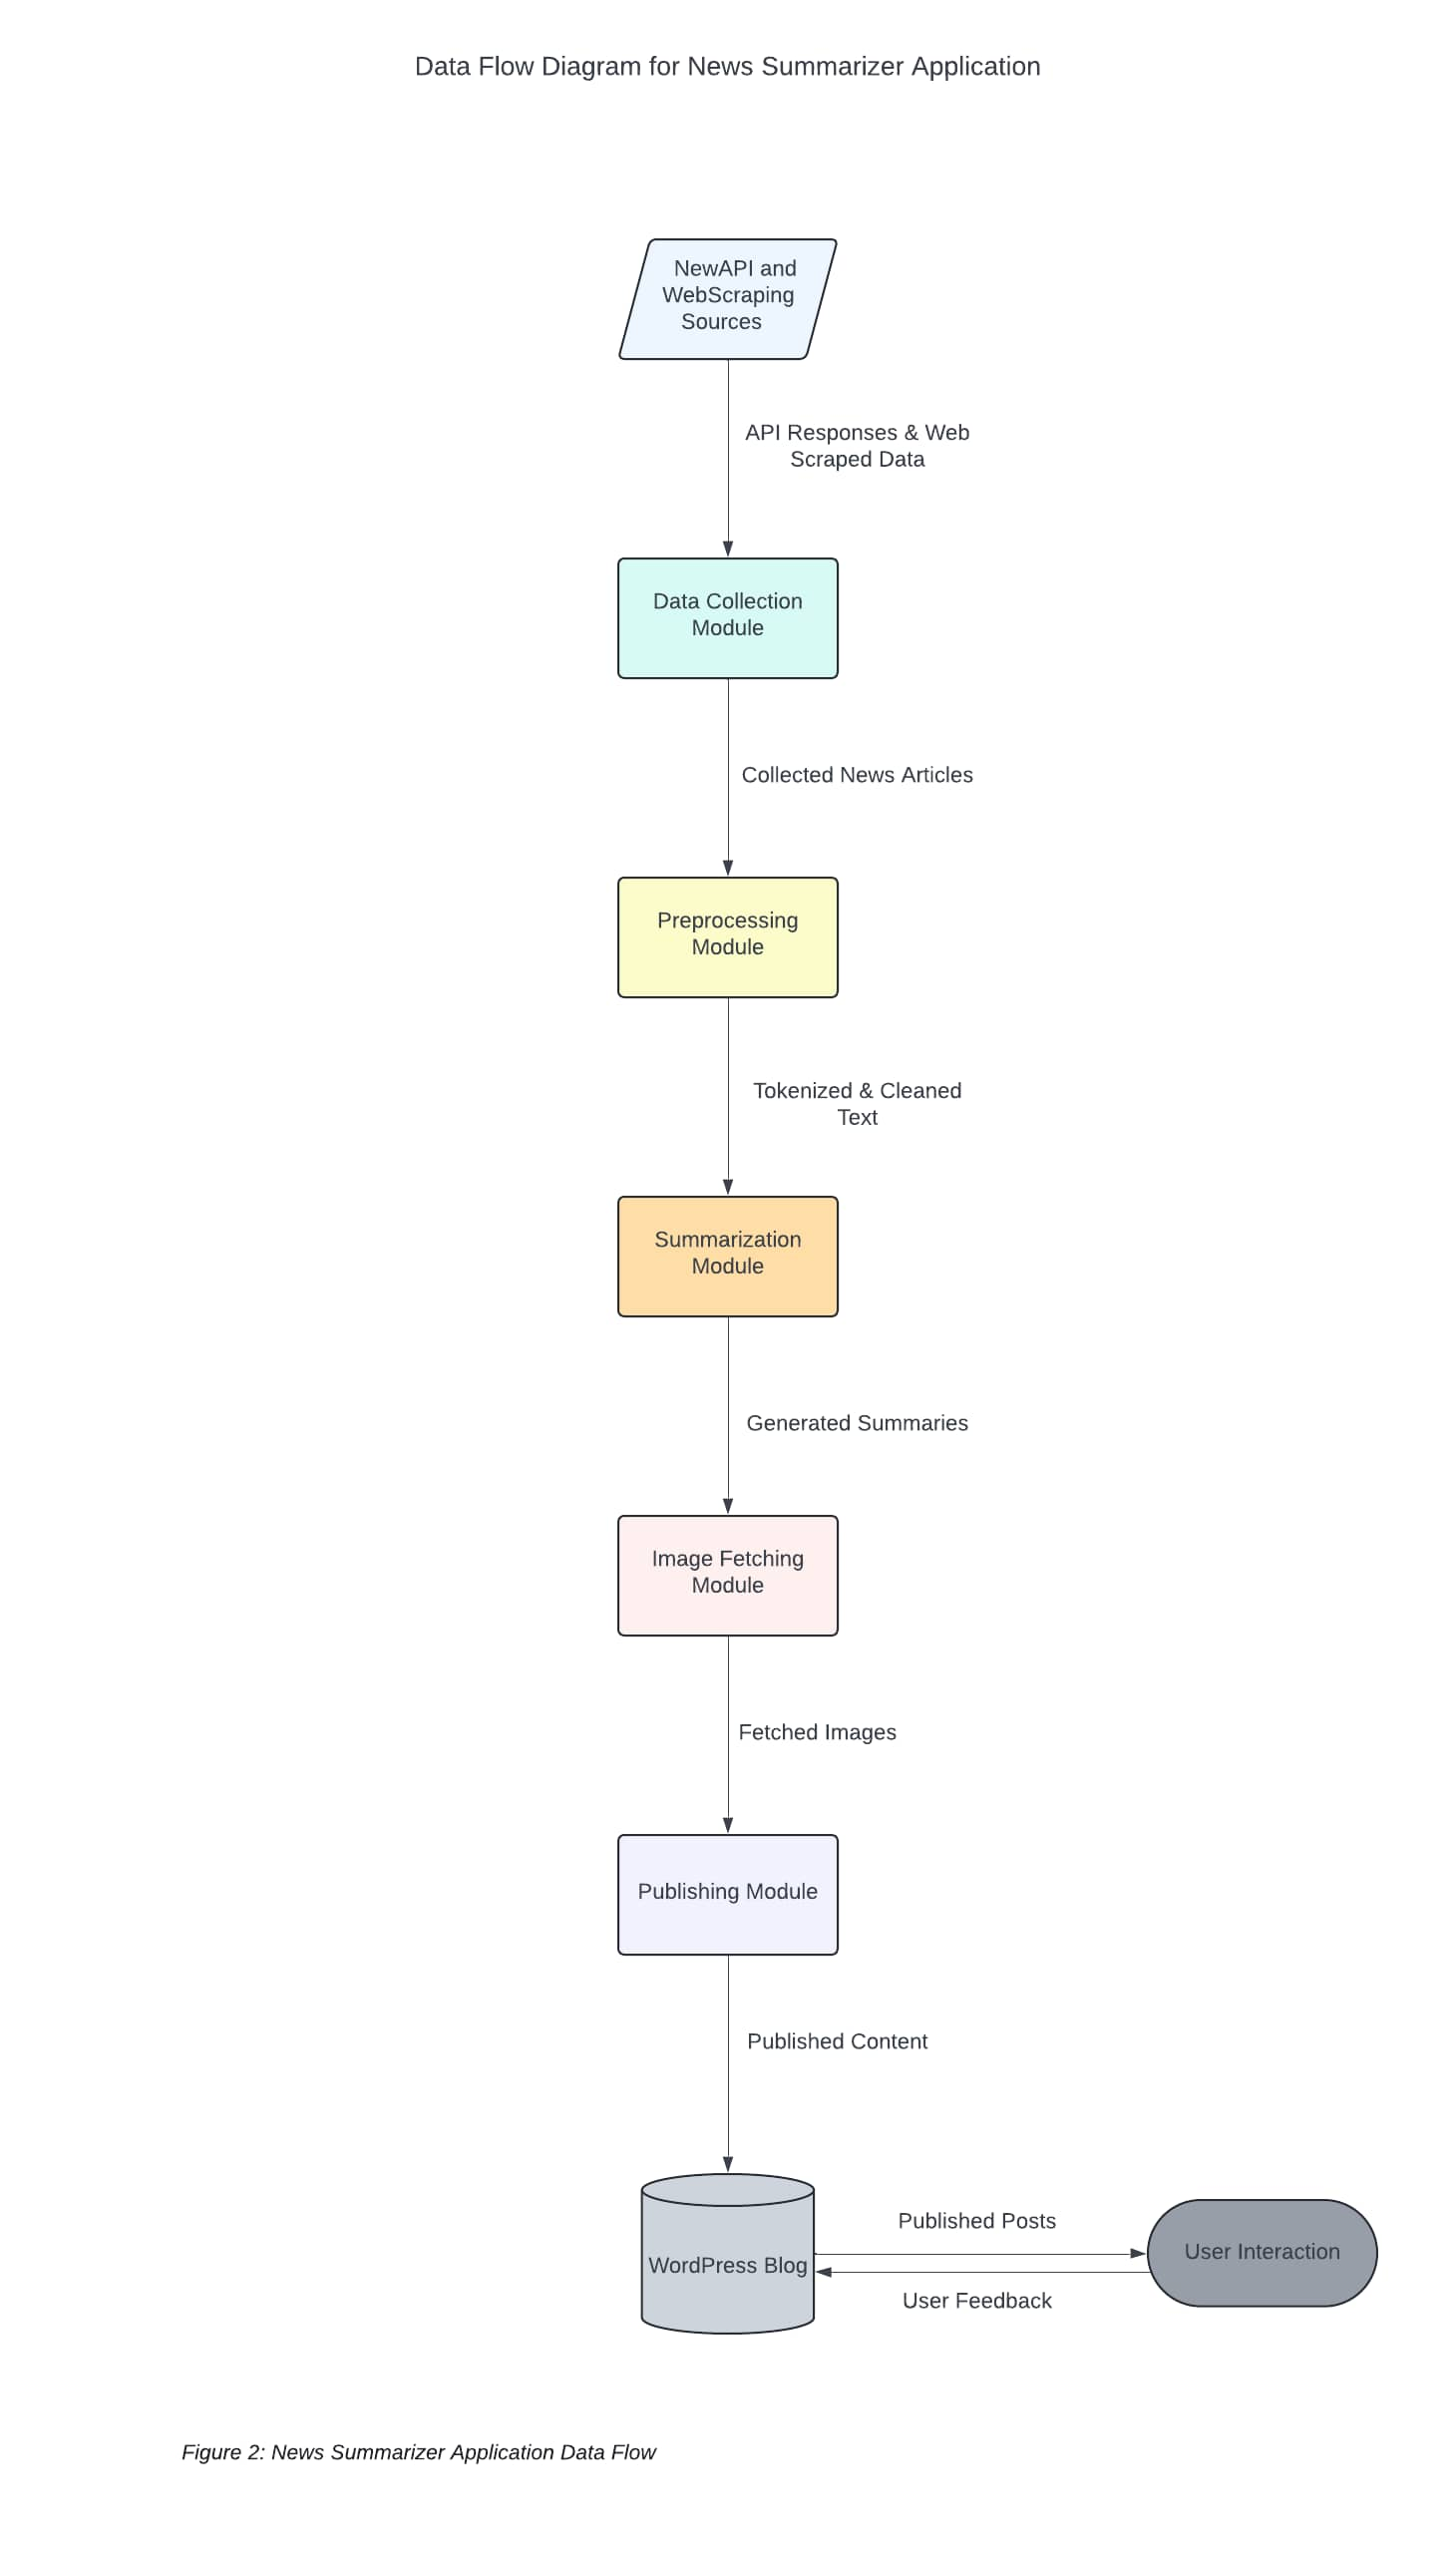
\includegraphics[width=0.7\textwidth]{freecompress-Copy of Data Flow Diagram for News Summarizer Application.png}
    \caption{News Summarizer Application Data Flow}
    \label{fig:dataflow}
\end{figure}

\subsection{Architecture Diagram}
The architecture diagram provides a high-level overview of the system components and their interaction.

\begin{figure}[htbp]
    \centering
    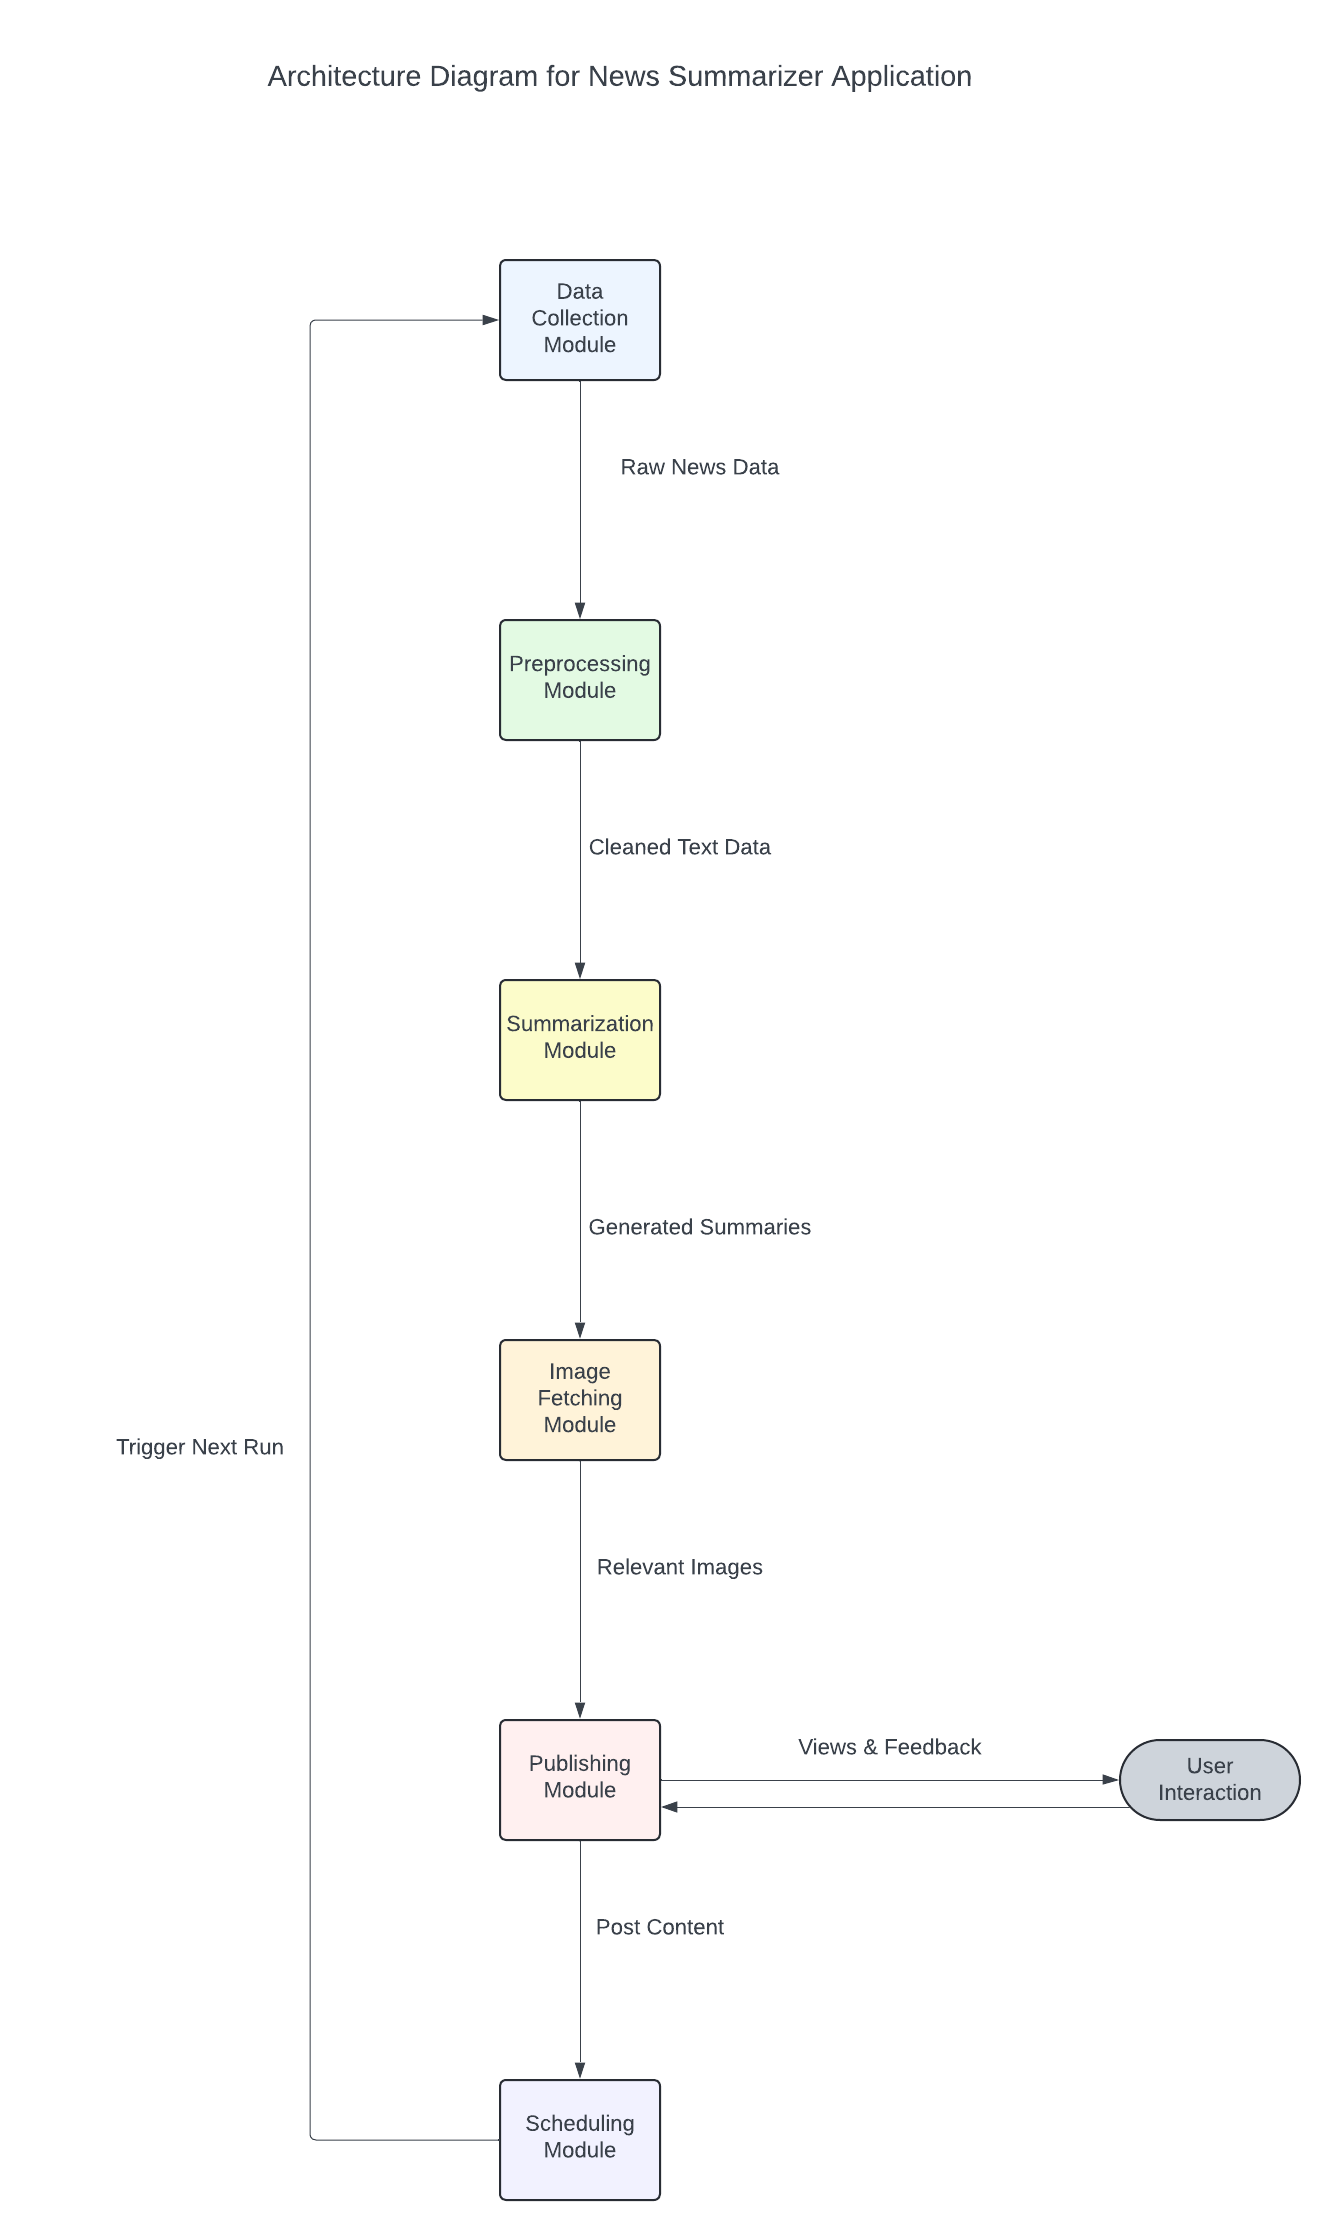
\includegraphics[width=0.61\textwidth]{Copy of Copy of Architecture Diagram for News Summarizer.png}
    \caption{News Summarizer Application Architecture}
    \label{fig:architecture}
\end{figure}
\newpage
\section{Evaluation}
To evaluate the system's performance, the generated summaries are compared to reference summaries using ROUGE (Recall-Oriented Understudy for Gisting Evaluation). This metric assesses the quality of both extractive and abstractive summarization models \citep{raffel2020exploring}. Abstractive models generally outperform extractive models, producing more coherent and human-like summaries. 

\begin{itemize}
    \item \textbf{ROUGE-N}: Measures the overlap of n-grams between the generated and reference summaries.
    \item \textbf{ROUGE-L}: Evaluates the longest common subsequence between the generated and reference summaries.
\end{itemize}

Human evaluation is also conducted to assess the readability and coherence of the summaries.

\section{Final Discussion}
\subsection{Strengths of the System}
\begin{itemize}
    \item \textbf{Efficiency}: The system quickly generates summaries, significantly reducing the time required to process and understand news content.
    \item \textbf{Scalability}: Capable of handling large volumes of articles from various news sources.
    \item \textbf{Flexibility}: The system supports both extractive and abstractive summarization techniques, allowing for flexibility in generating summaries for different use cases.
\end{itemize}

\subsection{Limitations}
\begin{itemize}
    \item \textbf{Complexity of Abstractive Models}: Abstractive summarization requires substantial computational power and is more difficult to fine-tune compared to extractive methods.
    \item \textbf{Data Sensitivity}: The quality of summaries is heavily dependent on the quality of the input data, particularly for news sources with poor-quality content or formatting issues.
\end{itemize}

\subsection{Recommendations}
\begin{itemize}
    \item \textbf{Model Updates}: Continuous updates and fine-tuning of transformer models are recommended to improve the system's performance.
    \item \textbf{Feedback Incorporation}: Regularly gathering feedback from users can help refine the quality of the generated summaries.
    \item \textbf{Additional Data Sources}: Expanding the sources of news articles will improve the system's coverage and accuracy.
\end{itemize}

\section{GitHub Repository}
All code and documentation for the implementation of this project are available in the following GitHub repository:
\href{https://github.com/stanleymay20/text-summarization-news-aggregation}{https://github.com/stanleymay20/text-summarization-news-aggregation}.

\section{Conclusion}
This paper presents an AI-based news summarization system that leverages both extractive and abstractive techniques to generate high-quality, concise summaries of news articles. The system is fully automated, from fetching articles to publishing summaries on WordPress. Our experiments demonstrate the system's effectiveness in handling large volumes of news data, and its successful deployment showcases its potential in real-world applications. Future work will focus on improving the abstractive summarization model and expanding the system to support more diverse news sources.

\bibliography{references}

\end{document}
